\documentclass[tikz,border=4pt]{standalone}

\usepackage{amsmath}
\usepackage{amssymb}
\usepackage{xcolor}
\usepackage{tikz}


\usetikzlibrary{
    arrows,
    arrows.meta,
    automata,
    backgrounds,
    calc,
    decorations.pathreplacing,
    fit,
    matrix,
    positioning,
    shapes,
    shapes.arrows,
    shapes.geometric,
    shapes.multipart
}



\tikzset{
  start/.style={
    rectangle,
    rounded corners,
    minimum width=3.5cm,
    minimum height=1cm,
    text centered,
    text width=3cm,
    draw=black,
    fill=green!20
  },
  stop/.style={
    rectangle,
    rounded corners,
    minimum width=3cm,
    minimum height=1cm,
    text centered,
    text width=2.5cm,
    draw=black,
    fill=red!20
  },
  decision/.style={
    diamond,
    aspect=2,
    minimum width=3cm,
    minimum height=1.2cm,
    text centered,
    text width=2.5cm,
    inner sep=1pt,
    draw=black,
    fill=yellow!20
  },
  process/.style={
    rectangle,
    minimum width=3cm,
    minimum height=1cm,
    text centered,
    text width=2.7cm,
    draw=black,
    fill=blue!10
  },
  arrow/.style={
    thick,
    -{Stealth}
  }
}


\usetikzlibrary{
  arrows.meta,
  positioning,
  shapes.geometric
}

\tikzset{
  start/.style={
    rectangle,
    rounded corners,
    minimum width=3.5cm,
    minimum height=1cm,
    text centered,
    text width=3cm,
    draw=black,
    fill=green!20
  },
  stop/.style={
    rectangle,
    rounded corners,
    minimum width=3cm,
    minimum height=1cm,
    text centered,
    text width=2.5cm,
    draw=black,
    fill=red!20
  },
  decision/.style={
    diamond,
    aspect=2,
    minimum width=3cm,
    minimum height=1.2cm,
    text centered,
    text width=2.5cm,
    inner sep=1pt,
    draw=black,
    fill=yellow!20
  },
  io/.style={
    trapezium,
    trapezium left angle=70,
    trapezium right angle=110,
    minimum width=3.5cm,
    minimum height=1cm,
    text centered,
    text width=3cm,
    draw=black,
    fill=blue!20
  },
  arrow/.style={
    thick,
    -{Stealth}
  }
}


\begin{document}

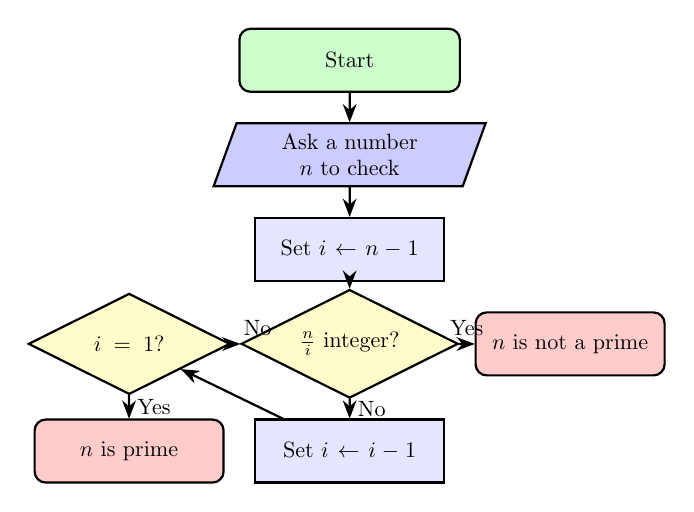
\begin{tikzpicture}[node distance=1.5cm, thick,scale=1.6, every node/.style={scale=0.8}]
    \node (start) [start] {Start};
    \node (input) [io, below of=start] {Ask a number $n$ to check};
    \node (seti) [process, below of=input] {Set $i \leftarrow n-1$};
    \node (ifdone) [decision, below of=seti] {$\frac{n}{i}$ integer?};
      \node (notprime) [stop, right of=ifdone, xshift=2.0cm] {$n$ is not a prime};
    \node (notdone) [process, below of=ifdone, yshift=-0.2cm] {Set $i \leftarrow i-1$};
    \node (iisone) [decision, left of=ifdone, xshift=-2.0cm] {$i=1$?};
      \node (prime) [stop, below of=iisone, yshift=-0.2cm] {$n$ is prime};

    \draw [arrow] (start) -- (input);
    \draw [arrow] (input) -- (seti);
    \draw [arrow] (seti) -- (ifdone);
    \draw [arrow] (ifdone) -- node[anchor=south] {Yes} (notprime);
    \draw [arrow] (ifdone) -- node[anchor=west] {No} (notdone);
    \draw [arrow] (notdone) -- (iisone);
    \draw [arrow] (iisone) -- node[anchor=west] {Yes} (prime);
    \draw [arrow] (iisone) -- node[anchor=south west] {No} (ifdone);
  \end{tikzpicture}

\end{document}
